\section{Framework Overview}\label{sec-arch}
The basic structure of SVC is: (1) given a query and a stale view, we construct a sample of the view, (2) from this sample we can estimate how updates affect the query result and compensate the result, and (3) we incorporate an index of outlier base table records to improve the accuracy of the results.
These three points map to the three main problems we address in this work, (1) formalizing this process as a data cleaning problem with the SampleClean framework, (2) defining a notion of row correspondence to link rows in the stale and updated views, and (3) outlier index.
In this section, we formalize these three problems and overview the architecture of SVC.

\subsection{Notation}
Given a database $\mathcal{D}$ which is a collection of relations $\{R_i\}$, a materialized view $S$ is the result of applying the relational expression $S_{def}$ to the database.
We use a multiset algebriac model (a set of elements with corresponding multiplicities) to represent the relations in the database $\mathcal{D}$ and the materialized view $S$.
We denote the multiset of insertions to a relation $R_i$ as $\Delta R_i$ and deletions as $\nabla R_i$.
In this paper, we refer to $\Delta R_i$ and $\nabla R_i$ as ``delta relations".
An update to a relation can be modeled as a deletion and then an insertion.
%In this work, we ignore \textbf{null} types and assume that each tuple in the relation has non-null attribute values.

We look at relation expressions for the view $S_{def}$ composed of the following operators:
\begin{itemize}\vspace{-.45em}
\item $\sigma_{\phi}(R)$: Selection select all tuples $r$ from $R$ that satisfy the restriction $\phi (r)$ \vspace{-.45em}
\item $\Pi_{a_1,a_2,...,a_k}(R)$: Projection select attributes $\{a_1,a_2,...,a_k\}$ from R \vspace{-.45em}
\item $\bowtie_{\phi (r1,r2)}(R_1,R_2)$: Join select all tuples in $R_1 \times R_2$ that satisfy $\phi (r_1,r_2)$.
\item $\gamma_{e}(R)$: Aggregation of R grouped by the relational expression $e(R)$.\footnote{A special case of this operator is $\delta$ the deduplication operator.}\vspace{-.45em}
\item $R_1 \dot{\cup} R_2$: Multiset union take a union of the two sets incrementing multiplicities.
\item $R_1 \dot{\cap} R_2$: Multiset intersection take an intersection of the set counting multiplicities.
\item $R_1 \dot{-} R_2$: Multiset set difference.
\end{itemize}

We denote the updated materialized view as $S'$, which is result of applying a maintenance strategy $\mathcal{M}$ defined in the previous section.

\subsection{Sampling}
In this work, we focus on uniform samples.
We define a sampling ratio $m\in [0,1]$ and for each row in a view $S$, we include it into a sample with probablity $m$.
Note, that this definition is slightly different from the reservoir sampling techniques studied in AQP which find a uniform
sample of \emph{size} $k\le \mid S \mid$.
To differentiate sampled relations from un-sampled ones we use the ``hat" notation eg. $\hat{S}$.

\subsection{Staleness and Freshness}
Given a materialized view $S$ and an updated materialized view $S'$.
In the deterministic case with no sampling, we call a query result $r = q(S)$ stale if:
\[r \ne q(S')\]
When there is sampling, this definition has to be made probabilistic.
\begin{definition} PROBABILISTIC STALENESS.
Let $\hat{S}$ be a uniform sample of $S$ with a sampling ratio of $m$,
and let $r_m$ be the result of applying $q$ to $\hat{S}$.
$r_m$ is \emph{stale} if and only if:
\[\lim_{m\rightarrow 1} r_m \ne q(S') \text{  a.s}\]

Conversely $r_m$ is \emph{fresh} for all values of $m$ if:
\[\lim_{m\rightarrow 1} r_m == q(S') \text{  a.s}\]
\end{definition}

\subsection{View Maintenance as Data Cleaning}
In SVC, we model this definition of staleness as a type of data error.
Materialized views whose base relations have been updated potentially give stale query results.
We formalize the problem of correcting staleness as a data cleaning operation.

If we are given a materialized view $S$ and we know the base relations have had insertions and deletions $U$, then given the operators defined earlier there are three possible types of error:
\begin{itemize}
\item A row in $S$ needs to be updated.
\item A row in $S$ needs to be deleted.
\item A new row needs to be inserted into $S$.
\end{itemize}

In this case, it is clear that simply executing the maintenance strategy $\mathcal{M}$ will acheive the necessary results and udpate the view $S$ to view $S'$.
However, now suppose we have a sampled view $\hat{S}$, and we want to do just enough effort to update only the rows in the that sample.
This problem is challenging since the errors are not just updates to rows in the views, as there might be new insertions needed.
Thus, we define cleaning in the following way: suppose we have a stale uniform sample $\hat{S}$ with sampling ratio $m$, we want to find an up-to-date uniform sample $\hat{S'}$.
We define the cleaning procedure as preserving the uniformity of sampling, so after cleaning $\hat{S'}$ is a uniform sample of $S'$:
\begin{itemize}
\item If an update is needed, update the row.
\item If the row needs to be deleted, delete the row.
\item For all new rows that need to be inserted into the view $S'$ insert a random sample of ratio $m$.
\end{itemize}

It is important to note that the way we defined data cleaning on a sample does not neccessary give a unique $\hat{S'}$. 
In this paper, we take advantage of this property and propose a technique that analyzes $\mathcal{M}$ and can find a particular $\hat{S'}$
efficiently.

\subsection{Efficient Maintenance of a Sample}
The input of this component is $S$ a stale view, a maintenance strategy $\mathcal{M}$, and the output is $\hat{S'}$.
The maintenance strategy is a relational expression the execution of which updates $S$.
The relational expression can be represented as a tree of relational operations. 
We add a sampling operator $\eta$, which uniformly samples rows from a relation, to the top of this tree.

We can see that this sampled maintenance strategy gives us the desired cleaning operation defined before.
However, as is, it is a naive implementation.
Placed at the top of the tree it would materialize $S'$ entirely then select those rows that happen to be in the sample.
In Section \ref{correction}, address this challenge by defining a set of push down rules for $\eta$ to maximize the operators that benefit from the sampling.

\subsection{Query Correction}
Given a query $q$ which has been applied to the stale view $q(S)$; thus the result is stale.
We want to calculate a $c$ such that $q(S)+c$ is fresh using the defition described previously.
The procedure to maintain a sample $\hat{S'}$ was described in the previous sub-section.
The correction $c$ is an estimate of how $\hat{S'}$ changed from $\hat{S}$.
The challenge is that we cannot use any uniform sample $\hat{S'}$ and uniform sample $\hat{S}$.
These samples must satisfy the following property, which we call \emph{correspondence}, and is a sort of an inverse to the 
data cleaning formalism defined earlier:

\begin{definition} CORRESPONDENCE.
The samples $\hat{S'}$ and $\hat{S}$ correspond if and only if:
\item For every row $r$ in $\hat{S}$ that required an update, $r\in \hat{S'}$
\item For every row $r$ in $\hat{S}$ that required a delete, $r \not\in \hat{S'}$
\end{definition}

Given this property of correspondence, we can apply \textbf{NormalizedSC}.
Like similar restrictions in other sampled-based systems \cite{agarwalknowing}, there are restrictions on the queries $q$ on the view that we can answer.
In this work, we extend beyond SampleClean's \sumfunc,\countfunc, and \avgfunc queries and consider general non-nested aggregate queries with simple predicates on a single view:
\begin{lstlisting} [mathescape]
SELECT $f(a)$ FROM View 
WHERE Condition(A);
\end{lstlisting}
We also consider correcting stale non-nested select queries of the following form with simple predicates:
\begin{lstlisting} [mathescape]
SELECT * FROM View 
WHERE Condition(A);
\end{lstlisting}
As with all sample estimates, for the estimates to be meaningful, the predicate should not be too selective. 
In this broader context, in Section \ref{sampling}, we discuss the semantics and guarantees for these queries.

\subsection{Outlier Indexing}
The correction $c$ in the previous subsection is derived from a sample.
Sampling is known to be senstive to outliers, which we define as records whose values deviate significantly from the mean.
However, a challenge is that since we do not materialize the entire up-to-date view detecting which records may be outliers is challenging.
Instead, we define an outlier index on base relations of the database $\mathcal{D}$.
This index tracks records whose attributes cross some threshold $t$.
Then, for a given view $S$, this component gives a series of rules to propagate the information from the outlier index upwards.
Basically, for every row in the view that is derived from a record in the outlier index, we ensure that it is incorporated into the sample.
We explore the conditions under which we can make this guarantee, and discuss query processing with the outlier index in Section \ref{outlier}.

\subsection{System Architecture}
In implementation, SVC works in conjunction with existing defered maintenance or re-calculation approaches.
We envision the scenario where materialized views are being refreshed periodically, for example nightly.
While maintaining the entire view throughout the day may be infeasible, sampling allows the database to scale the cost with the performance and resource constraints during the day.
Then, between maintenance periods, we can provide approximately up-to-date query results for some queries.
We illustrate this setup in Figure \ref{sys-arch}.

\subsection{Example Application: Log Analysis}
Without getting into the specific technical details, to illustrate our system and justify our argument about performance improvements, we use the following running example which is a 
simplified schema of one of our experimental datasets (Figure~\ref{example-1}).
Imagine, we are querying logs from a video streaming company. 
These logs record visits from users as they happen and grow over time.
We have two tables, \tbl{Log} and \tbl{Video}, with the following schema:

\begin{lstlisting}[mathescape]
Log(sessionId$\textrm{,}$ videoId$\textrm{,}$ responseTime$\textrm{,}$ userAgent)
Video(videoId$\textrm{,}$ title$\textrm{,}$ duration)
\end{lstlisting}
These tables are related with a foreign-key relationship between
Log and Video, and there is an integrity constraint that every log
record must link to one video in the Video table.

\begin{figure}[ht!] 
\centering
\vspace{-0.75em}
 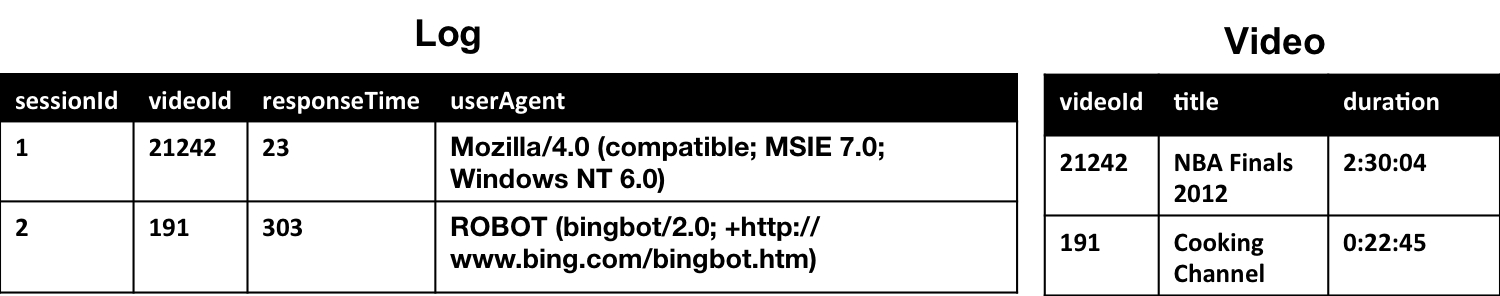
\includegraphics[width=\columnwidth]{figs/sample-clean-example.png}\vspace{-0.25em}
 \caption{A simplified log analysis example dataset. In this dataset, there are two tables: a fact table representing video views and a dimension table representing the videos.\label{example-1}}
\end{figure}

Consider the following example materialized view, which finds a count of the number of times the video's loading latency was greater than 10\% of the duration of the view:

\vspace{0.5em}

\begin{lstlisting} 
SELECT videoId, 
count(1) AS slowResponseTimes 
FROM Log, Video
WHERE Log.videoID = Video.videoID and
	  responseTime > .1*Video.duration
GROUP BY videoId;
\end{lstlisting}

The user wants to know how many videos repeatedly have slow responses.
\begin{lstlisting} 
SELECT COUNT(1)
FROM AggView
WHERE slowResponseTimes > 100;
\end{lstlisting}
Let us suppose the initial query result is $45$.
There now have been new log records inserted into the Log table making the old result stale.
For example, if our sampling ratio is 5\%, that means for 5\% of the videos (distinct videoID's) we refresh stale slowResponseTimes if necessary.
From this sample, we calculate how many new videos changed from a slowResponseTimes of less than 100ms to times greater than 100ms; let us suppose this answer is $2$.
Since our sampling ratio is 5\%, we extrapolate that $40$ new videos throughout the view should now be included in the count.
This means that we should correct the old result by $40$ resulting in the estimate of $85$.

\iffalse
We add the following operator $\eta_{a_1, m}(R)$ which is the \textbf{hash} operator.
For all tuples in R, this operator applies a hash function whose range is $[0,1]$ to attribute $a_1$ and selects those records with hash value less than or equal to $m$.
%We make two assumptions on this hash operator: (1) \emph{independence} there is no expression in $S_{def}$ that is dependent on the hash operator, and (2) \emph{uniformity} over the domain of possible attribute values the \emph{a priori} probability of including any tuple is the same.
Finally, we use the \emph{query tree} representation to analyze $S_{def}$ where we unravel composed relational operators into a tree of expressions.
Each leaf of the tree is a relation and each node is an operator.



\subsection{Semantics of Query Results}
We should note that there is an implicit design tradeoff in the way we formulated this problem.
By sampling the maintenance plans, our approach is very general with respect to supported views.
On the other hand, we are restricted in the types of queries that we can run.
If we were to sample from the delta relations instead, this tradeoff would be flipped. 
We have a further discussion about this subtlty in Section ??.

A important concern of users is what are the semantics and guarantees on their corrected query results.
In Table ??, we list all of the aggregate queries supported by Apache HiveQL present a taxonomy of result semantics for these queries.
We will detail the corrections to these queries in Section \ref{correction}.
\fi